\documentclass[10pt]{article}

\usepackage[margin=1in]{geometry}
\usepackage[T1]{fontenc}
\usepackage[utf8]{inputenc}
\usepackage{lmodern}
\usepackage{amsmath,amssymb,mathtools}
\usepackage{booktabs}
\usepackage{tabularx}
\usepackage{array}
\usepackage{graphicx}
\usepackage{caption}
\usepackage{float}
\usepackage{enumitem}
\usepackage{microtype}
\usepackage{xcolor}
\usepackage{natbib}
\usepackage[hidelinks]{hyperref}

\setlength{\parindent}{1em}
\setlength{\parskip}{0.25em}
\setlist{nosep,leftmargin=*}
\captionsetup{font=small,labelfont=bf}
\newcolumntype{Y}{>{\centering\arraybackslash}X}

\title{HyperChE: Normalized Hypergraph Retrieval for High-Order Chemical Facts}
\author{Anonymous Authors}
\date{}

\begin{document}
\maketitle

\begin{abstract}

Chemical literature often expresses a useful result as a high-order fact: a material or formulation is evaluated under particular composition and operating conditions, produces one or more measurements, and is associated with a performance outcome. These roles may be distributed across chunks or repeated with different names and units. Chunk retrieval preserves the original wording but provides a coarse retrieval unit, while pairwise graph representations can weaken the binding between conditions, measurements, and outcomes. We present \textbf{HyperChE}, a chemical-domain retrieval-augmented generation (RAG)~\citep{RAG,RAGsurvey} pipeline that organizes this evidence with a normalized hypergraph. HyperChE combines entity and relation normalization, explicit measurement and condition instances, canonical/surface dual representations, and hybrid entity--hyperedge retrieval with deterministic candidate reranking. On a frozen dataset, we evaluate five retained systems using the same evaluation view. HyperChE performs better than the original hypergraph and the chemistry-prompted pairwise-graph comparison. The paper reports the contribution of chemistry-domain prompting, normalization, complete-fact coverage, and the final group's candidate organization and reranking under a shared protocol.

\textbf{Keywords:} chemical information retrieval; retrieval-augmented generation; hypergraph; knowledge representation; entity normalization; high-order facts

\end{abstract}
\section{Introduction}

Chemical literature often places a material or formulation, its composition and operating conditions, measurements, and a property or performance outcome in one experimental claim. These roles may be distributed across text chunks or repeated with different names and units. A text chunk preserves the original wording, while an independently indexed pairwise relation may fail to keep conditions, measurements, and outcomes bound to the same experimental instance. We call this multi-role, jointly constrained evidence a \textbf{high-order chemical fact}. A hyperedge can bind the material, components, condition instances, measurements, outcome, and source location into one retrievable record.

HyperChE's retrieval and question-answering flow has three steps. First, the question is encoded and used to search separate entity and hyperedge indexes, with canonical forms supporting matching across aliases and relation variants while surface forms remain available for evidence tracing. Second, the retrieved entity and hyperedge lists are fused with weighted reciprocal rank fusion (RRF); matched entities are expanded through their incident facts, the structured candidates are mapped back to source chunks, and a deterministic structural reranker may be applied. Third, the leading evidence chunks, their fact roles, and their source pointers are passed to a QA generator, which produces a grounded answer with citations when the evidence supports one. Fact extraction, normalization, and index construction are offline preparation steps for this online flow.

We organize the study around three design questions and one evaluation-boundary question:

\begin{itemize}
\item \textbf{RQ1 -- Chemical-domain prompting:} What role does a chemistry-domain extraction prompt play in constructing and retrieving pairwise graphs and hypergraphs? Is its effect the same for the two representations?
\item \textbf{RQ2 -- Normalization and coverage:} Does entity and relation normalization improve retrieval quality and recovery of complete facts? We use both ranking metrics and Composite Fact Recall (CFR).
\item \textbf{RQ3 -- Final-system advantage:} Where does the advantage of the final normalized hypergraph come from? When F0 and F1 share a candidate pool, does structural reranking improve ordering, and does it add new complete facts?
\item \textbf{RQ4 -- Generation and boundaries:} How does evidence coverage appear in supplementary QA, and which protocol factors limit the strength of the conclusions?
\end{itemize}

The evaluation uses 60 documents, 1,328 frozen chunks, 58 queries, 4,196 judged query--chunk pairs, and 150 accepted atomic facts. The retained systems are B0 (original hypergraph), B1 (chemistry-prompted pairwise graph), B2 (chemistry-prompted hypergraph), F0 (normalized hypergraph without reranking), and F1 (normalized hypergraph with reranking).

\section{Related Work and Problem Positioning}

\subsection{Chemical information extraction and knowledge graphs}

Chemical information extraction must represent more than named entities. A useful record may include material identity, composition, synthesis or operating conditions, a measurement with a unit and interval, a comparison target, and a reported property or performance outcome. The same concept may appear under abbreviations, spelling variants, trade names, alternate unit conventions, or context-dependent relation phrases. A knowledge representation that only stores an entity string and a generic relation can therefore merge mentions that should remain distinct or detach a measurement from the condition under which it was obtained.

Knowledge graphs provide a practical abstraction for indexing entities and relations, and chemical knowledge graph systems have enabled search, prediction, and synthesis-oriented applications. Their common representation is a collection of typed entities and pairwise edges. This representation is valuable for many tasks, particularly when a fact is naturally binary or when graph traversal is the main operation. For the retrieval problem considered here, however, a chemical observation may be jointly constrained by more than two participants and by attached measurements and conditions. The challenge is to preserve that scope while still supporting efficient matching and source-level inspection.

HyperChE treats normalization as part of the representation rather than as a post-processing cosmetic step. Canonical forms support aggregation and retrieval across aliases, relation variants, units, and numerical forms. Surface forms and evidence pointers remain available for citation, audit, and reconstruction of the original claim. Measurement and condition instances are represented as roles within a fact record so that values from separate experimental settings are not silently converted into unconditional properties.

\subsection{Retrieval-augmented generation and graph-augmented retrieval}

Standard retrieval-augmented generation (RAG)~\citep{RAG,RAGsurvey} usually indexes document chunks and supplies the top-ranked passages to a language model. This design is simple and preserves local prose, but a chunk is a coarse retrieval unit: it may contain several facts, omit a condition located in a neighboring chunk, or return a phrase without exposing the relations that connect it to the question. Under a query/chunk relevance protocol, chunk retrieval can also have a structural advantage because a directly returned chunk already contains the answer wording.

Graph-augmented RAG introduces entities, relations, communities, or paths as additional retrieval and reasoning structures. GraphRAG~\citep{GraphRAG} and subsequent systems use graph construction, entity retrieval, graph expansion, or path-based ranking to improve the organization of large corpora. Other systems specialize graph interfaces for particular domains or combine graph evidence with chunk retrieval. These methods show that structured retrieval can complement the local context of conventional RAG.

The relevant distinction for HyperChE is the retrieval unit and the evidence-assembly operation. A pairwise graph exposes local edges and neighborhoods. A hypergraph exposes the entities and roles that belong to one n-ary fact, allowing an entity match to expand to a complete fact or a fact match to expose all its members. HyperChE therefore uses hybrid retrieval to generate candidates but evaluates whether the returned evidence supports complete accepted facts, rather than only whether one local phrase is relevant.

\subsection{Hypergraph knowledge representation}

A standard graph is commonly written as

\[
G=(V,E),
\]

where $V$ is a set of entities and each edge in $E$ connects two endpoints. A pairwise fact can be written with an endpoint tuple $V_e=(v_h,v_t)$. A hypergraph generalizes this structure as

\[
G_H=(V,E_H),
\]

where each hyperedge $e_H\in E_H$ connects two or more entities,

\[
V_{e_H}=(v_1,v_2,\ldots,v_n),\qquad n\geq 2.
\]

The corresponding n-ary fact is

\[
F_n=(e_H,V_{e_H})\in G_H.
\]

The $n=2$ case contains an ordinary edge as a special case. The point of the generalization is not merely to increase the number of edges. It changes the unit that can be stored, retrieved, expanded, and inspected: a hyperedge can represent the joint membership of several entities in one fact. HyperGraphRAG~\citep{HyperGraphRAG} first makes this loss of binding intuitive by showing one concrete fact in three forms--chunk text, binary graph edges, and a hyperedge--and then gives the formal definition. It subsequently constructs a knowledge hypergraph, retrieves entities and hyperedges, expands the retrieved structure in both directions, and combines the recovered facts with chunk evidence.

For chemical applications, this order of explanation is useful. A material--component--condition--measurement--outcome record can first show how pairwise decomposition fragments a fact; the formal definition then states what the hyperedge preserves. An implementation may use a bipartite incidence graph or another database structure for storage. The storage choice itself does not reduce the semantic representation to binary facts when hyperedge membership is preserved losslessly.

Prior hypergraph representation and hyper-relational embedding work has often focused on link prediction, node classification, or representation learning. HyperChE addresses a different operational goal: retrieving source-grounded evidence for questions about chemical experiments. The central measurements are therefore retrieval ranking and complete-fact coverage, with QA as a supplementary check on whether retrieved evidence can support a generated answer.

\subsection{Evaluation of chemical RAG systems}

This paper evaluates HyperChE from three perspectives: retrieval ranking, complete-fact coverage, and question answering. Hit@5, MRR, and gNDCG@5 represent the ranking quality of relevant evidence; Composite Fact Recall measures whether the system retrieves evidence that fully supports a chemical fact; and QA metrics show how the retrieved evidence affects the final answer. Source diversity is reported as an auxiliary diagnostic.

\subsection{Problem positioning and study scope}

HyperChE lies at the intersection of chemical information extraction, graph-augmented RAG, and hypergraph knowledge representation. We separate three design questions that are often conflated: whether a chemistry-domain prompt is needed, whether normalization improves retrieval and complete-fact recall, and where the advantage of the final configuration comes from. We therefore examine whether a pipeline combining domain prompting, normalization, measurement and condition modeling, canonical/surface traceability, and entity--hyperedge retrieval can improve high-order evidence recovery under a shared protocol.

The retained experiments provide five system views: the original hypergraph (B0), the chemistry-prompted pairwise graph (B1), the chemistry-prompted unnormalized hypergraph (B2), the normalized hypergraph without reranking (F0), and the normalized hypergraph with deterministic reranking (F1). B1 and B2 are system-level comparisons because their retrieval entrances and candidate organization differ; F0 and F1 share the same hybrid RRF top-50 candidate pool and differ only in the post-generation reranking switch.

\section{Problem Definition}

\subsection{Task formulation and design goals}

HyperChE is designed for retrieval over chemical literature in which a useful answer is often determined by a combination of entities, measurements, operating conditions, and outcomes. The retrieval target is therefore not only an isolated entity or a locally matching sentence. It is an evidence set that preserves the binding among the roles that jointly define a chemical fact.

Let $q$ be a query and let $R_k(q)$ be the ranked list of the top-$k$ source chunks returned by the system. The system is evaluated at two levels. At the chunk level, a returned chunk is relevant when it satisfies the shared query--chunk judgment protocol. At the fact level, a composite fact is supported only when its exact supporting chunk appears in $R_k(q)$. The second level prevents a system from receiving full credit merely for returning a related entity while missing the condition, measurement, or result that completes the fact.

The design has four goals:

\begin{enumerate}
\item preserve multi-role chemical facts as retrievable units;
\item make aliases, relation variants, and measurement expressions searchable under a common representation;
\item retain the original surface wording so that retrieved evidence can be traced back to the source text; and
\item separate candidate recall from candidate ordering so that the contribution of deterministic reranking can be measured.
\end{enumerate}

\subsection{Ordinary graphs and hypergraphs}

An ordinary graph is written as

\[
G=(V,E),
\]

where $V$ is a set of nodes and each edge $e\in E$ connects two endpoints, for example $e=(v_h,v_t)$. This representation is appropriate for a binary relation, but a chemical statement can require more than two jointly constrained roles. For example, the statement that a material under a specified operating condition has a measured value and a corresponding performance result cannot be fully characterized by one isolated pairwise edge without distributing the condition and measurement over additional edges.

HyperChE uses a hypergraph

\[
G_H=(V,E_H),
\]

where a hyperedge $e_H\in E_H$ is incident to a set of two or more nodes,

\[
V_{e_H}=(v_1,v_2,\ldots,v_n),\qquad n\geq 2.
\]

The associated high-order fact is represented as

\[
F_n=(e_H,V_{e_H}).
\]

An ordinary edge is therefore the $n=2$ case, whereas a hyperedge can keep the material, component, condition, measurement, property, and outcome of one fact in a common incidence scope. The implementation may store the incidence relation as a bipartite edge--entity structure for indexing. This storage choice does not reduce the semantic unit to an independent collection of binary facts: the hyperedge identity, its member set, its typed roles, and its evidence pointer are retained together.

\section{HyperChE Method}

\subsection{Chemical fact extraction and evidence binding}

The input corpus is divided into frozen source chunks. A domain-specific extraction pass produces, for each chunk, entity mentions, relation or fact descriptions, measurement instances, condition instances, and pointers to the source evidence. The extraction record is organized around a fact instance rather than around an unconstrained list of entity pairs. A useful abstract form is

\[
f_i=(s_i,r_i,A_i,M_i,C_i,P_i,E_i),
\]

where $A_i$ is the set of participating entities, $M_i$ is the set of measurements, $C_i$ is the set of conditions, $P_i$ contains the property or outcome roles, and $E_i$ identifies the source chunk and evidence span. The role sets may be partially populated when the source statement does not provide every role; the system does not fill missing roles by combining unrelated chunks.

Measurements are kept as typed local instances. A measurement may include a value or interval, a unit, a comparator, and the object to which the value applies. Conditions are kept as instances as well, so that temperature, composition, flow, loading, or other operating context remains attached to the fact in which it was observed. Values that are ambiguous in the chunk-local extraction are preserved rather than silently split or assigned to a different object. This prevents a value observed under one condition from becoming an unconditional property of the material.

The extraction record also stores the original surface wording and an evidence pointer. These two fields serve different purposes: the structured record supports matching and aggregation, while the surface evidence supports quotation, reconstruction, and manual audit.

\subsection{Entity and relation normalization}

Chemical literature uses aliases, abbreviations, spelling variants, unit variants, and relation phrases that refer to the same underlying concept. HyperChE maps such variants to a canonical representation before indexing. Normalization is applied to entity names, relation descriptions, and measurement or unit expressions when a canonical form is available. The source surface form is retained alongside the canonical form.

Let $x^{\mathrm{surf}}$ denote a mention as it appears in the source and $x^{\mathrm{can}}$ its normalized form. The dual record is

\[
\operatorname{Dual}(x)=
\bigl(x^{\mathrm{can}},x^{\mathrm{surf}},E_x\bigr),
\]

where $E_x$ is the evidence pointer. Canonical text makes equivalent mentions easier to aggregate across chunks and documents. Surface text preserves the wording needed to verify a result and to reconstruct the source chunk. The final cache uses the \texttt{dual\_concat} index profile so that both views remain available to the retrieval representation; the exact surface string is never discarded from the evidence record.

Normalization is not treated as an independent semantic label. It is a representation and indexing operation whose value is tested through the end-to-end retrieval and composite-fact results. The final cache records the normalization version and an evidence rewrite audit, allowing the canonical record and its source form to be checked independently.

\subsection{Hypergraph construction and indexed objects}

Each normalized fact is represented by a hyperedge-like relationship object and a set of incident entity nodes. The relationship object contains the canonical relation text, surface description, typed role information, the measurement and condition instances, and the source pointer. Entity objects contain canonical and surface names plus their incident relationship identifiers. The resulting incidence structure supports two complementary retrieval views:

\begin{itemize}
\item \textbf{entity view:} retrieves entities whose canonical or surface descriptions match the query;
\item \textbf{relationship view:} retrieves binary or higher-arity relationship objects whose fact descriptions match the query.
\end{itemize}

The same source chunk can therefore be reached from an entity match, a relationship match, or both. After graph expansion, the system reconstructs the complete source chunk rather than exposing only a truncated graph fragment to the generator. This keeps graph retrieval connected to verifiable textual evidence.

\subsection{Hybrid candidate retrieval}

For a query $q$, HyperChE independently computes dense and lexical scores for relationship objects and entity objects. The candidate lists are fused with weighted reciprocal rank fusion (RRF). For a candidate $d$, the fusion score has the form

\[
S_{\mathrm{RRF}}(d)=
\sum_{j\in\mathcal{L}(d)}
\frac{w_j}{k_{\mathrm{RRF}}+\operatorname{rank}_j(d)},
\]

where $\mathcal{L}(d)$ is the set of dense or BM25 lists containing $d$, $w_j$ is the channel weight, and $k_{\mathrm{RRF}}$ is the RRF offset. The final normalized retrieval configuration uses relationship dense and BM25 channels, entity dense and BM25 channels, one-hop incident-edge expansion, and a deterministic structural rerank over a frozen candidate pool. Relationship candidate depth is 50, entity candidate depth is 30, the RRF offset is 60, and the relationship and entity channel weights are fixed by the released protocol. These settings are held constant between the no-rerank and rerank variants.

One-hop expansion follows incident relationships from retrieved entities and adds their linked fact objects, subject to the released expansion limit. The resulting candidate pool is mapped back to source chunks. If multiple structured objects map to the same chunk, the chunk is retained once with its associated structured evidence. The final ranked output is a list of reconstructed source chunks, which is the unit used by the shared qrels and by the QA evidence interface.

\section{Experimental Setup}

\subsection{Corpus, queries, and frozen artifacts}

The evaluation uses a fixed chemical literature collection from the flow-battery domain. The collection contains 60 documents and 1,328 frozen source chunks produced with a configured chunk length of 1,000 characters. The retrieval test set contains 58 queries. The shared candidate pooling and judgment process covers 4,196 query--chunk pairs, and every retained pair has a fixed relevance judgment. The composite-fact audit contains 150 manually accepted atomic facts.

The released final cache contains 11,950 entity records, 13,629 relationship records, and 14,676 audited evidence instances. These counts describe construction and audit artifacts; they are not substitutes for retrieval-quality metrics. The complete experiment directory retains the raw experiment outputs, while the paper database stores the retained systems, accepted qrels, fact audit, and derived summaries.

All retained systems use \texttt{Qwen/Qwen3-Embedding-4B} with 2,560 embedding dimensions for embedding-based retrieval. The original caches are treated as read-only inputs.

\subsection{Main systems}

The main results retain five systems, with fixed names and roles:

\begin{table}[t]
\centering
\small
\begin{tabularx}{\linewidth}{Xrr}
\toprule
Group & System & Role in the paper \\
\midrule
B0 & \texttt{original\_hypergraph} & Original hypergraph baseline \\
B1 & \texttt{chem\_prompt\_graph} & Chemistry-prompted pairwise-graph comparison \\
B2 & \texttt{chem\_prompt\_hypergraph} & Chemistry-prompted, unnormalized hypergraph comparison \\
F0 & \texttt{normalized\_final\_no\_rerank} & Normalized hypergraph with reranking disabled \\
F1 & \texttt{normalized\_final} & Final normalized hypergraph with deterministic reranking \\
\bottomrule
\end{tabularx}
\end{table}

B0--B2 are retained as system-level comparisons and should not be read as strict one-factor ablations: the historical systems differ in extraction, indexing, candidate adapters, and text realization. In particular, B1 and B2 use different candidate-organization procedures. The B2 result is therefore interpreted as a diagnostic of its released, unnormalized hypergraph retrieval protocol, rather than as evidence that hypergraphs are intrinsically inferior to pairwise graphs.

F0 and F1 form the controlled ablation. They share one normalized cache, embedding model, hybrid RRF candidate process, and fixed top-50 candidate pool; the only difference is the deterministic structural reranking switch.

\subsection{Retrieval protocol}

The primary relevance threshold is grade $\geq 2$, with grade $\geq 3$ reported as a stricter sensitivity threshold. Shared qrels use four relevance grades, 0--3. Every retained system is evaluated on the same judged query--chunk set. The main metrics are:

\begin{itemize}
\item \textbf{P@1:} the proportion of queries whose first result reaches the selected relevance threshold;
\item \textbf{Hit@5:} the proportion of queries with at least one threshold-reaching result in the top five;
\item \textbf{MRR:} the mean reciprocal rank of the first threshold-reaching result;
\item \textbf{shared gNDCG@5:} graded NDCG computed from shared judgments, with IDCG calculated separately for each query; and
\item \textbf{Composite Fact Recall@5 (CFR@5):} the fraction of the 150 accepted atomic facts whose exact supporting chunk appears in the top five.
\end{itemize}

The shared-IDCG construction gives every retained system the same per-query denominator. Five queries have no usable IDCG under the fixed judgment set; they follow the released zero-denominator handling rule and are disclosed in the metric notes. This paper version does not include confidence intervals or formal hypothesis tests, so it does not use statistical-significance language or claim statistical superiority.

CFR is intentionally stricter than ordinary Hit@5. It requires the exact supporting chunk for an accepted atomic fact to appear; a related chunk or a chunk that matches an entity but lacks the fact's condition and outcome does not count as complete support. \texttt{macro\_query\_CFR@5} is reported as a supplementary query-level summary when needed. Source-level fields in the archive are derived from chunk qrels and are diagnostic rather than an independently annotated source-level gold standard.

\subsection{Supplementary QA protocol}

QA is a supplementary check of how retrieved evidence is used. The fixed question set contains 40 questions, 35 answerable and 5 unanswerable. The generator receives the top five retrieved chunks with a 1,500-character evidence budget. Generation uses \texttt{kimi-k2.6}, temperature 1.0, top-$p$ 0.95, and seed 20260811. EFU repair remains disabled.

The final normalized system uses an Alibaba Cloud DashScope service for generation and judging. Historical QA runs for the other retained systems use a Moonshot service. Although the nominal model name is the same, the providers and service conditions differ. QA values are therefore reported as supplementary evidence and are not presented as a fully controlled five-system generation ranking. The primary conclusions rely on retrieval metrics and CFR, which use shared qrels and the fixed fact audit.

This boundary is part of the result interpretation. The question studied here is whether structured and normalized hypergraph evidence improves retrieval of high-order chemical facts under a fixed structured-evidence protocol. The conclusions are limited to the retained systems, fixed corpus, query set, and shared evidence judgments.

\section{Results and Discussion}

\begin{figure}[t]
\centering
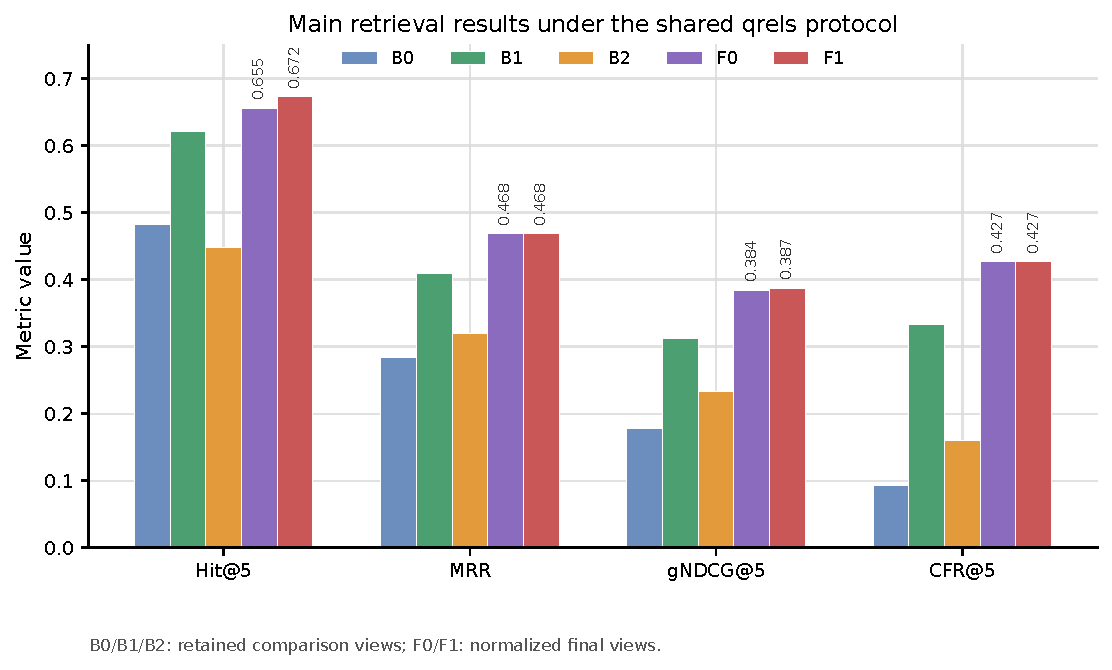
\includegraphics[width=0.92\linewidth]{figures/main_results_four_metrics.pdf}
\caption{Primary retrieval and complete-fact results for the five retained systems. Each panel uses the shared grade-$\geq2$ evaluation view.}
\label{fig:main-results}
\end{figure}
\subsection{Results}

\subsubsection{RQ1: Is chemistry-domain prompting necessary?}

We evaluate five retained systems on a fixed collection of 60 chemical documents and 1,328 chunks. The benchmark contains 58 retrieval queries and 4,196 judged query--chunk pairs, each with a final relevance grade. The main retrieval results use the shared $\mathrm{IDCG}@5$ protocol and report relevance at grade $\geq 2$. The five systems are:

\begin{itemize}
\item \textbf{B0 (original hypergraph):} the original hypergraph cache and retrieval implementation;
\item \textbf{B1 (chemistry-prompted graph):} a chemistry-prompted pairwise graph;
\item \textbf{B2 (chemistry-prompted hypergraph):} a chemistry-prompted hypergraph without the final normalization and evidence-organization pipeline;
\item \textbf{F0 (normalized hypergraph, no reranking):} the normalized final cache with reranking disabled; and
\item \textbf{F1 (normalized hypergraph):} the normalized final cache with the deterministic structural reranker enabled.
\end{itemize}

Composite Fact Recall (CFR) uses the same 150 accepted atomic facts. A fact counts as supported only when its exact supporting chunk is retrieved in the top five. This criterion is intentionally stricter than ordinary chunk relevance: it measures whether the retrieved set contains a complete, directly usable evidence unit.

Relative to B0, the chemistry-prompted systems show that a domain prompt changes the retrieval representation and yields gains on some metrics, but the effect is not uniform across adapters. B1 raises grade-$\geq 2$ Hit@5 from 0.4828 to 0.6207. B2 reaches 0.4483 on this metric but raises CFR from 0.0933 to 0.1600. Because B1 and B2 use different upstream retrieval adapters, these comparisons answer whether the prompted system configurations are useful; they do not identify a prompt-only causal effect. Chemistry-domain prompting is therefore a design factor that must be tested rather than a component whose benefit can be assumed in advance.

\subsubsection{RQ2: Does normalization improve retrieval quality?}

Table 1 reports grade-$\geq 2$ retrieval performance. F1 obtains the best result on every primary ranking metric retained for the main comparison.

\begin{table}[t]
\centering
\small
\begin{tabularx}{\linewidth}{Xrrrr}
\toprule
System & P@1 & Hit@5 & MRR & gNDCG@5 \\
\midrule
B0: original hypergraph & 0.1897 & 0.4828 & 0.2832 & 0.1779 \\
B1: chemistry-prompted graph & 0.2759 & 0.6207 & 0.4091 & 0.3122 \\
B2: chemistry-prompted hypergraph & 0.2241 & 0.4483 & 0.3194 & 0.2329 \\
F0: normalized hypergraph, no reranking & 0.3276 & 0.6552 & 0.4683 & 0.3842 \\
F1: normalized hypergraph & \textbf{0.3276} & \textbf{0.6724} & \textbf{0.4684} & \textbf{0.3873} \\
\bottomrule
\end{tabularx}
\end{table}

The final normalized system improves substantially over B0. Hit@5 increases from 0.4828 to 0.6724 (+18.97 percentage points), MRR from 0.2832 to 0.4684 (+0.1852), and gNDCG@5 from 0.1779 to 0.3873 (+0.2094). Compared with B1, the strongest retained pairwise-graph comparison, F1 is higher by 5.17 percentage points in Hit@5, 0.0593 MRR points, and 0.0751 gNDCG points. At the stricter grade-$\geq 3$ threshold, F1 reaches Hit@5 = 0.5690, compared with 0.5345 for B1, 0.3793 for B2, and 0.3621 for B0. Under the current judgment scale, F1's advantage is therefore not limited to lower-grade relevant chunks.

These results support the bounded claim that the normalized hypergraph pipeline is effective for the present chemical high-order-fact retrieval task. They do not imply that every hypergraph implementation is better than every pairwise graph. In particular, B2 is below B1, which shows that representation and retrieval must be designed together.

\subsubsection{RQ2 continued: Does normalization improve complete-fact recall?}

CFR provides a complementary view of whether retrieved evidence preserves a complete chemical fact rather than only a locally relevant fragment.

\begin{table}[t]
\centering
\small
\begin{tabularx}{\linewidth}{Xrrr}
\toprule
System & Supported facts / 150 & CFR@5 & Macro query CFR \\
\midrule
B0: original hypergraph & 14 & 0.0933 & 0.1963 \\
B1: chemistry-prompted graph & 50 & 0.3333 & 0.3213 \\
B2: chemistry-prompted hypergraph & 24 & 0.1600 & 0.2011 \\
F0: normalized hypergraph, no reranking & 64 & 0.4267 & 0.4324 \\
F1: normalized hypergraph & \textbf{64} & \textbf{0.4267} & \textbf{0.4324} \\
\bottomrule
\end{tabularx}
\end{table}

F1 supports 64 of the 150 accepted facts, compared with 14 for B0 and 50 for B1. Its CFR is 0.4267, versus 0.3333 for B1 and 0.0933 for B0. This is the clearest evidence that the final pipeline improves coverage of complete, multi-role facts under the exact-supporting-chunk criterion. At the same time, 86 of the 150 facts are still not fully supported in the top five. The remaining gap indicates that cross-chunk evidence aggregation, candidate diversity, and retrieval of conditions with weak lexical cues remain unresolved.

CFR and Hit@5 should be interpreted together. Hit@5 can improve when one relevant fragment is retrieved, whereas CFR requires the exact supporting chunk for an accepted atomic fact. The higher F0/F1 CFR therefore indicates a change in evidence coverage, not only a change in the ordering of individually relevant chunks.

\subsubsection{RQ3: Where does the final-system advantage come from?}

The final-system advantage can be considered at three levels: normalized fact representation, hybrid candidate organization and recall pool, and ordering after candidate generation. The following analysis separates these levels as far as the available experiments allow.

\paragraph{Why B2 is below B1}

The B2 result should not be interpreted as evidence that hypergraph structure is intrinsically inferior to a pairwise graph. B1 and B2 are not a strict one-variable ablation; their upstream retrieval adapters differ in several operational respects.

B1 uses a structured graph hybrid pipeline with entity dense retrieval, entity BM25, relationship dense retrieval, relationship BM25, weighted reciprocal-rank fusion, and incident-edge expansion. It does not impose a fixed quota between entity and relationship branches. B2 uses the upstream \texttt{hyper\_query} interface, which returns separate entity and relation branches, takes ten results from each, interleaves them, and applies a top-20 cutoff while preserving branch order. It therefore has a fixed 10+10 allocation and lacks an equivalent to B1's multi-channel fusion and expansion.

The candidate diagnostics are consistent with this explanation. Before the final branch quota and top-20 cutoff, the B2 candidate union has higher gold recall than B1 (0.8889 versus 0.8222). After B2's quota and truncation, its effective candidate recall falls to 0.5333, with 16 query-level quota or top-k losses. B1 has no corresponding quota loss in this diagnostic. Several B2 queries contain a gold entity or relation at a rank outside the fixed branch budget, so the relevant candidate is discarded even though it appears in a broader branch union.

Candidate text form may also contribute. B2 represents complete hyperedges with multiple entities, relation descriptions, and evidence text. Under the current BM25 and candidate-text construction, these longer descriptions can dilute query terms and push a relevant hyperedge lower in a branch ranking. This is an implementation-level explanation, not a theoretical property of hypergraphs. The current B2 top-20 diagnostic also selects no high-order candidate in the returned set, so this adapter does not measure the full potential of high-order retrieval.

Accordingly, B2 is treated as a chemistry-prompted hypergraph baseline without the final reconstruction and normalization pipeline, with its limitations reported explicitly. A strict structural ablation would make B1 and B2 share the same dense/BM25/RRF/expansion pipeline, candidate budget, textualization procedure, and reranking policy, changing only the relation arity restriction. That controlled experiment is left for future work.

\begin{figure}[t]
\centering
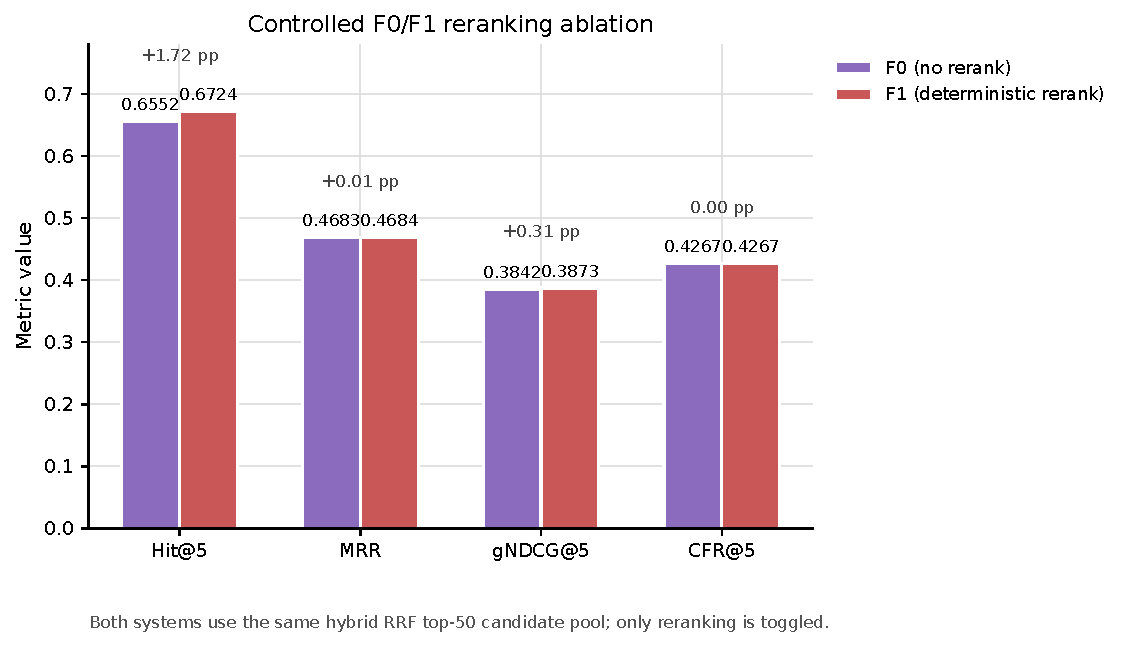
\includegraphics[width=0.78\linewidth]{figures/f0_f1_rerank_ablation.pdf}
\caption{F0/F1 reranking ablation under the shared hybrid RRF top-50 candidate pool.}
\label{fig:rerank}
\end{figure}
\subsubsection{RQ4: What does reranking add after candidate generation?}

F0 and F1 use the same hybrid RRF top-50 candidate pool. Their only intended difference is whether the deterministic structural reranker is applied after candidate generation.

\begin{table}[t]
\centering
\small
\begin{tabularx}{\linewidth}{Xrrr}
\toprule
Metric & F0 (no reranking) & F1 (reranking) & Difference \\
\midrule
P@1 & 0.3276 & 0.3276 & 0.0000 \\
Hit@5 & 0.6552 & 0.6724 & +0.0172 \\
MRR & 0.4683 & 0.4684 & +0.0001 \\
gNDCG@5 & 0.3842 & 0.3873 & +0.0031 \\
CFR@5 & 0.4267 & 0.4267 & 0.0000 \\
\bottomrule
\end{tabularx}
\end{table}

Reranking yields a small top-five boundary improvement: Hit@5 increases by 1.72 percentage points and gNDCG@5 by 0.0031. MRR changes by only 0.0001, while CFR remains 0.4267. Fixing the candidate pool at top 50 means F1 cannot introduce a fact that was absent from those candidates. It does not, however, make CFR invariant: reordering can move an exact-support chunk into or out of the top five. In this experiment the observed CFR is equal for F0 and F1, indicating that no additional exact-support chunks crossed the evaluated top-five boundary.

This ablation separates two effects. The main improvement over B0 and B1 is associated with normalized representation and the hybrid candidate-generation process. The current reranker supplies a limited ordering refinement rather than a new source of fact coverage. Future gains should prioritize candidate recall, cross-chunk aggregation, and source diversity before additional ranking complexity.

\subsubsection{Evidence-source diversity and failure patterns}

As a diagnostic derived from chunk-level qrels, F1 retrieves an average of 2.121 distinct source documents in its top five, with a duplicate ratio of 0.576. F0 has 2.103 distinct sources and a duplicate ratio of 0.579. B0, B1, and B2 have respectively 3.586/0.283, 2.897/0.421, and 3.621/0.276 for these two quantities.

The lower source diversity of F0/F1 indicates that higher chunk-level relevance is sometimes obtained by repeatedly retrieving evidence from the same source. This concentration is compatible with the unchanged F0/F1 CFR: reranking can promote a relevant chunk from an already retrieved source without increasing the number of independently supported facts. These source statistics are descriptive diagnostics computed from chunk qrels; they are not an independently annotated source-level gold standard.

The retained per-query inspection identifies three recurring failure patterns:

\begin{enumerate}
\item \textbf{Missing cross-chunk evidence:} one part of a fact is retrieved, but the condition or outcome needed to establish the complete fact is absent from the top five;
\item \textbf{Condition-binding errors:} a material or performance value is retrieved without the operational condition that scopes it; and
\item \textbf{Incomplete comparison pairing:} evidence for one side of a comparison is retrieved while the corresponding material, baseline, or measurement for the other side is missing.
\end{enumerate}

These patterns explain why a system can obtain a relevant top-ranked chunk while still failing the stricter composite-fact criterion.

\subsubsection{QA as a supplementary result and protocol boundary}

The final QA run contains 40 questions: 35 answerable and 5 explicitly unanswerable. It uses top-$k=5$ retrieved evidence, a 1,500-character evidence budget, temperature 1.0, top-$p=0.95$, and seed 20260811.

\begin{table}[t]
\centering
\small
\begin{tabularx}{\linewidth}{Xr}
\toprule
QA metric & F1 \\
\midrule
Good Rate & 0.2500 \\
Satisfactory-or-Better Rate & 0.5000 \\
Macro KPC & 0.4633 \\
Micro KPC & 0.4825 \\
Hallucination Rate & 0.2000 \\
False Abstention Rate & 0.1714 \\
False Answer Rate & 0.0000 \\
Unanswerable Abstention Accuracy & 1.0000 \\
Citation Reference Validity & 1.0000 \\
Citation Presence Rate & 0.7250 \\
Citation Support Score & 0.4649 \\
\bottomrule
\end{tabularx}
\end{table}

Half of the questions reach satisfactory-or-better quality, and all generated citations are valid under the QA audit. The false-answer rate is zero, but the hallucination and false-abstention rates show that incomplete evidence still limits answer completeness and calibration. QA therefore serves as a consistency check for the retrieval analysis rather than a replacement for retrieval evaluation.

\subsection{Discussion}

\subsubsection{What the results say about chemical hypergraph retrieval}

Chemical literature often states a result through a joint constraint over several roles: a material or component, a composition, an operating condition, a measurement or range, and a performance outcome. The retrieval objective is not merely to find a chunk mentioning one of these terms; it is to preserve the binding that makes the combination a usable fact.

The F1 results are consistent with this view. Relative to B0 and B1, F1 retrieves more complete atomic facts under the exact-supporting-chunk criterion and improves conventional ranking metrics. The evidence supports using a hypergraph-oriented organization for this class of facts when it is coupled with domain normalization and an appropriate retrieval adapter. It does not support the stronger claim that hypergraph structure alone guarantees improvement.

\subsubsection{Normalization is a retrieval mechanism, not only data cleaning}

Normalization in the final pipeline is a retrieval mechanism, not merely data cleaning. Entity and relation variants are normalized, measurement and condition instances are modeled, and canonical and surface forms are retained together. Canonical forms allow aliases, units, and relation variants to match during retrieval and aggregation; surface forms preserve original wording and evidence pointers for citation and audit. The difference between B2 and F1 is best interpreted as a system-level transition from an unnormalized, quota-constrained hypergraph adapter to a normalized, evidence-oriented retrieval pipeline. The present results cannot isolate each component because extraction, indexing, textualization, candidate fusion, and representation change together. They do show that high-order representation becomes more useful when entities, relations, measurements, conditions, and evidence pointers are organized consistently.

\subsubsection{Recall and ranking should be improved in that order}

The F0/F1 comparison shows that reranking is not the main observed source of gain. F0 already reaches CFR@5 = 0.4267, equal to F1, while F1 provides only a modest Hit@5 improvement. Once a complete fact is absent from the candidate pool, a downstream ranker cannot recover it. Candidate generation, cross-chunk links, and source diversity should therefore be prioritized before more ranking complexity. The source-diversity diagnostic also suggests a trade-off: F1's top five are more concentrated within the same source than B1 or B2, which may help local relevance but reduce the chance of collecting complementary evidence from different sections or papers.

\subsubsection{Interpreting the pairwise-graph comparison}

B1 is a useful retained comparison because it is a strong chemistry-prompted pairwise graph, but its result also reflects a different retrieval adapter. The B2 diagnosis shows that candidate quotas and ranking behavior can dominate the observed outcome before the representation itself is evaluated. The main conclusion is therefore framed around the complete normalized pipeline: F1 is stronger than the retained baselines under the shared qrels protocol, while B2 shows that hypergraph representation and retrieval must be co-designed.

\subsubsection{QA interpretation and practical meaning}

QA shows a useful but incomplete transfer from retrieval to generation. Valid citations and a zero false-answer rate indicate an auditable evidence interface, while the Good Rate of 0.25 and Hallucination Rate of 0.20 show that evidence coverage and fact binding still constrain practical answer quality. Historical QA used Moonshot and F1 used Alibaba Cloud DashScope, so the QA values are supplementary rather than a fully controlled generation ranking.

\subsubsection{Scope of the claim}

The evidence supports four bounded conclusions:

\begin{enumerate}
\item On this fixed chemical benchmark, the normalized hypergraph pipeline improves retrieval quality over the retained original hypergraph, chemistry-prompted pairwise graph, and chemistry-prompted hypergraph baselines.
\item Under the accepted exact-supporting-chunk CFR protocol, it recovers more complete atomic facts in the top five than those baselines.
\item The deterministic reranker provides a small ordering benefit after candidate generation but does not increase complete-fact coverage in this experiment.
\item For chemical literature with condition-coupled facts, hypergraph structure is useful when combined with normalization, fact-role organization, candidate fusion, and evidence textualization; structure alone is not sufficient.
\end{enumerate}

\section{Limitations}

Hypergraph construction adds engineering and computational cost. The system requires multi-entity relation extraction, entity and relation normalization, measurement and condition instance modeling, hyperedge--entity--source-evidence linking, and synchronized entity and hyperedge indexes. These steps increase offline model calls, manual auditing, storage, and index-maintenance costs. When documents are updated, the affected facts, normalization mappings, and evidence pointers may need to be checked again. Online queries also perform entity and hyperedge retrieval, incident-fact expansion, source-chunk reconstruction, and candidate reranking, making the workflow more complex than a single text index. The present study does not quantify build time, service cost, storage overhead, or incremental-update cost.

\section{Conclusion}

Chemical literature often expresses knowledge as a combination of material, composition, operating condition, measurement, and performance outcome. These roles jointly constrain the meaning of a fact, and their association can be weakened when the fact is represented only as independent pairwise relations or retrieved as an unstructured text block. HyperChE addresses this problem with a normalized hypergraph representation that preserves high-order fact membership, measurement and condition instances, and a dual view of canonical matching forms and surface evidence.

On the fixed evaluation set, the final normalized system reaches grade-$\geq 2$ Hit@5 = 0.6724, MRR = 0.4684, shared gNDCG@5 = 0.3873, and Composite Fact Recall@5 = 0.4267. The corresponding original-hypergraph values are 0.4828, 0.2832, 0.1779, and 0.0933. The CFR increase is especially relevant: it indicates that the final system retrieves more complete atomic-fact support, rather than only improving isolated chunk matching.

These results support a bounded conclusion: on this chemical benchmark and under this shared protocol, a normalized hypergraph is a useful way to organize high-order chemical knowledge. The result depends on normalization, role-aware fact organization, candidate retrieval, and evidence binding; it should not be generalized to every hypergraph implementation or every chemical corpus without further controlled evaluation.

\appendix
\section*{Appendix}

The appendices follow the reproducibility-oriented organization used by HyperGraphRAG: prompt interfaces, construction and retrieval algorithms, data and judgments, evaluation protocol, configuration, detailed audit outputs, construction cost, and the reproducibility manifest. They describe only the retained HyperChE systems.

\section{Chemical fact extraction and query interfaces}

\subsection{Extraction interface}

The offline extraction prompt asks the model to segment each frozen source chunk into self-contained chemical fact records. The output schema preserves:

\begin{itemize}
\item a fact or relationship description;
\item entity mentions with role, surface form, and canonical form when available;
\item measurement instances with value or interval, unit, comparator, and measured object;
\item condition instances such as composition, temperature, flow, loading, or operating mode;
\item property or outcome roles;
\item source chunk identifier and evidence span; and
\item an extraction completeness or uncertainty field when the source statement is incomplete.
\end{itemize}

The prompt keeps roles that belong to the same experimental statement together and leaves unavailable roles empty. It must not fill a missing condition or result by combining unrelated chunks. Service credentials are never part of the prompt or paper package.

\subsection{Query parsing interface}

The online query parser returns structured search cues rather than an answer: entity and material mentions, relation or outcome terms, measurement and unit cues, condition terms, normalized aliases when available, and the original query text for evidence tracing. The parser keeps the input language and does not invent a chemical fact. Subsequent entity and hyperedge retrieval can use canonical and surface forms together.

\subsection{Evidence-grounded QA interface}

The QA interface receives the query and the reconstructed top-five source chunks. The prompt requires an answer supported by the supplied evidence, citations or source pointers when available, and explicit abstention when evidence is insufficient. QA does not perform EFU repair, retrieve extra evidence, or silently fill missing conditions. The fixed generation configuration is given in Appendix D.

\section{HyperChE construction and online retrieval}

\subsection{Offline construction}

Input: frozen document collection D For each source chunk: extract chemical fact records and evidence spans normalize entities, relations, measurements, and units retain canonical and surface forms create a typed-role hyperedge fact object link the fact object to incident entities and source chunks store incidence structures and evidence pointers build dense and lexical indexes for entities and fact objects audit normalization rewrites and cache integrity Output: normalized HyperChE cache

A bipartite incidence structure is used as the storage representation. The semantic object remains the fact object together with its member set, typed roles, and evidence pointer.

\subsection{Online retrieval and generation}

Input: query q encode q and retrieve entity and fact-object candidates from dense and lexical indexes fuse lists with weighted RRF expand retrieved entities through incident fact objects map structured candidates back to source chunks construct the common hybrid RRF top-50 candidate pool apply the deterministic reranker only for F1 pass the top-five reconstructed chunks to the QA interface Output: ranked evidence and an optional grounded answer

F0 and F1 use the same candidate pool. The only switch between them is the deterministic structural reranking stage after candidate generation. A fixed top-50 pool prevents the reranker from adding candidates outside that pool, but it does not make top-five metrics mathematically invariant.

\subsection{Construction and retrieval complexity}

Let $D$ be the number of documents, $r$ the maximum number of extracted facts per document, and $n$ the maximum number of entities or typed roles per fact. Under a constant prompt-cost assumption per document, extraction requires model calls proportional to $D$. Fact-object insertion is $O(Dr)$, incidence writes are bounded by $O(Drn)$, and embedding the final entity and fact-object sets requires $O(|V|+|E_H|)$ encoder calls. These are structural upper bounds; actual wall-clock cost depends on token length, batching, retries, and index implementation.

For a query, dense or lexical lookup has a linear-scan upper bound of $O(|V|+|E_H|)$. One-hop expansion is bounded by $O(kd)$, where $k$ is the retrieved candidate count and $d$ is the average incident degree. Source reconstruction and deterministic reranking add costs proportional to candidate-pool size and evidence length. Approximate nearest-neighbor indexes can reduce practical lookup cost.

\section{Dataset, qrels, and Composite Fact Recall}

The frozen evaluation contains 60 chemical documents, 1,328 source chunks, 58 queries, 4,196 judged query--chunk pairs, and 150 user-accepted atomic facts. The source chunks and query files are frozen before comparing the retained systems.

Shared qrels use four grades, 0--3. The primary threshold is grade $\geq 2$, with grade $\geq 3$ as a stricter sensitivity view. Every retained system uses the same judged query--chunk set and the same per-query IDCG denominator. Five queries have no usable IDCG under the frozen judgment set and follow the released zero-denominator handling rule.

Composite Fact Recall at $k$ is defined over the 150 accepted atomic facts. An atomic fact is counted as supported only when its exact supporting source chunk appears in the top-$k$ result list. A related chunk, matching entity, or partial condition does not count as complete support. Source-level hit and diversity fields are derived from chunk qrels and are diagnostic rather than independently annotated source-level gold.

The audit package contains the accepted fact file, qrels audit, and derived CFR summaries. The full 4,196-row qrels table is kept as a supplementary artifact rather than embedded in the paper body.

\section{Evaluation and QA protocol}

All retained systems use Qwen/Qwen3-Embedding-4B with 2,560 embedding dimensions. Original caches are read-only inputs and EFU repair is disabled throughout retrieval and QA.

The retained system views are:

\begin{table}[t]
\centering
\small
\begin{tabularx}{\linewidth}{Xr}
\toprule
System & Configuration \\
\midrule
B0 & Original hypergraph \\
B1 & Chemistry-prompted pairwise graph \\
B2 & Chemistry-prompted, unnormalized hypergraph \\
F0 & Normalized hypergraph with reranking disabled \\
F1 & Normalized hypergraph with deterministic reranking \\
\bottomrule
\end{tabularx}
\end{table}

The normalized retrieval configuration uses entity and relationship dense and BM25 channels, one-hop incident-fact expansion, relationship candidate depth 50, entity candidate depth 30, and RRF offset 60. F0 and F1 share the hybrid RRF top-50 candidate pool; F1 applies the deterministic structural reranker after candidate generation.

In the released configuration, relationship dense and BM25 channel weights are 1.0 and entity dense and BM25 channel weights are 0.8. The expansion weight is 0.9, expansion depth is one hop, the maximum expanded fact-object count is 100, and the chunk candidate depth is 30. The final QA run uses three parallel workers with 120-second model and embedding timeouts.

Retrieval metrics are P@1, Hit@5, MRR, shared gNDCG@5, and Composite Fact Recall@5. QA is supplementary and uses 40 questions, 35 answerable and 5 unanswerable, top-$k=5$, a 1,500-character evidence budget, temperature 1.0, top-$p$ 0.95, and seed 20260811. F1 uses an Alibaba Cloud DashScope service, while historical QA records use a Moonshot service. The provider difference is disclosed and the QA values are not treated as a fully controlled generation ranking.

\section{Detailed results and audit slices}

The main tables report aggregate metrics for the retained systems. The supplementary package provides the following auditable views without duplicating every row in the paper:

\begin{enumerate}
\item per-query ranked outputs and threshold hits;
\item shared-IDCG inputs and zero-denominator cases;
\item Composite Fact Recall mappings from accepted facts to exact supporting chunks;
\item slices by fact arity, support mode, question type, and difficulty;
\item F0/F1 candidate-boundary changes under the shared top-50 pool; and
\item representative failure categories.
\end{enumerate}

The recurring failure categories are missing cross-chunk evidence, incorrect condition binding, and incomplete comparison pairing. These cases explain why a relevant top-ranked chunk does not always constitute complete fact support. Supplementary files include \texttt{shared\_retrieval\_per\_query\_retained.csv}, \texttt{shared\_retrieval\_ranked\_topk\_retained.csv}, \texttt{shared\_qrels\_final\_audit.json}, \texttt{composite\_fact\_gold\_user\_accepted.json}, \texttt{composite\_fact\_recall\_retained.csv}, and the QA summary files in the paper database.

\subsection{Representative evidence-assembly case}

The audit package contains QA\_RFB\_001, a cross-section question asking whether post-cycling capacity loss in a methyl-viologen flow cell is better explained by intrinsic 3-TMA PROXYL degradation or by self-discharge. The accepted evidence comes from source document RFB\_002 and two exact chunks, RFB\_002\_CHK\_001 and RFB\_002\_CHK\_009. The fact has arity 4 and support mode \texttt{cross\_section}. The accepted interpretation combines post-cycling diagnostic results, the lack of strong evidence for irreversible degradation, and evidence for self-discharge or crossover. This case shows why a single related sentence is insufficient: the answer requires evidence from multiple sections while keeping the material, condition, diagnostic measurement, and mechanism bound to the same question.

\section{Hypergraph construction cost and maintenance}

Construction cost has four components: LLM extraction and retry tokens, normalization and evidence-rewrite work, embedding calls for entities and fact objects, and storage and index construction. When a document is updated, the affected chunks may need to be re-extracted, aliases and units re-normalized, incident links regenerated, and corresponding dense and lexical index entries refreshed. Incremental maintenance is therefore more expensive than appending an unstructured text record.

The current experiment records structural counts and protocol settings but does not claim a complete monetary cost or end-to-end wall-clock benchmark. A future cost table should report extraction tokens, embedding calls, build time, index size, update time, and query latency separately, making the accuracy--cost trade-off explicit.

\section{Reproducibility manifest and data inventory}

The paper database contains protocol records, frozen query and qrels artifacts, accepted-fact audits, retrieval summaries, QA summaries, and source-level diagnostic files. Principal files include:

\begin{itemize}
\item \texttt{hyper\_final\_experiment\_v1\_state.json};
\item \texttt{hyper\_final\_posthoc\_v1\_run\_config.json};
\item \texttt{shared\_qrels\_final\_audit.json};
\item \texttt{composite\_fact\_gold\_user\_accepted.json};
\item \texttt{composite\_fact\_recall\_retained.csv};
\item \texttt{shared\_retrieval\_summary\_retained.json}; and
\item \texttt{qa\_final\_protocol.json} and \texttt{qa\_final\_summary\_normalized\_final.json}.
\end{itemize}

The final arXiv package should include the code version, cache version, query-file hash, qrels-audit hash, embedding model and dimension, retrieval settings, QA settings, and appendix tables. API keys and other secrets must not appear in the paper, source archive, or reproducibility package.


\bibliographystyle{plainnat}
\input{references.bbl}

\end{document}
